\graphicspath{{images/}}

\section{\thesection~Discussion}
\label{sec:discussion}

Fitness ranking from competition model fits may be better than from
logistic model fits (Will comparing stripes rankings reveal
anythin?). However, we cannot quantitatively compare fitness estimates
between plates because we are not finding global minima. Work has
begun to develop a genetic algorithm to do so. I am not convinced that
this will succeed because growth is systematically overestimated when
we move from the filled to striped plate for all of the current best
parameter solutions. This suggests an issue with the modelling
approach; below I suggest ways in which this could be improved. In
any case, qualitative cross-plate validation using order of fitness
ranking may still be better (for the competition model).

The first thing to notice about QFA data - from P15, the striped
plate, and the filled plate - is the characteristic endpoint in growth
on each plate (experiments could be designed to study variation in
timescales over regions of a plate by inoculating cultures in columns
left-to-right according to fitness). This suggests a plate-level or
region-level growth-limiting effect.
% This could conceivably be an experimental limitation such as the
% drying out of an agar plate over time.
Comparison of the striped and filled data, shows that cultures grow
larger when neighbours are removed and this suggests a direct
interaction between cultures. The strongest candidates are competition
for nutrients and growth limiting signalling such as ethanol
poisoning. It is possible that other growth limiting effects may exist
and could confound any attempt to fit a model which accounts for just
one of these. It makes sense to investigate each likely effect in turn
to determine its contribution and to start by validating the
independent limit.



Spots can grow after a long time. Must be nutrients remaining or an
encroachment? I have an image for the stripes plate showing cultures
growing and believe after a very late stage. I need to check the data
images but this may just be encroachment of another culture.
\graphicspath{{images/stripes/}}
\begin{Figure}
  \centering
  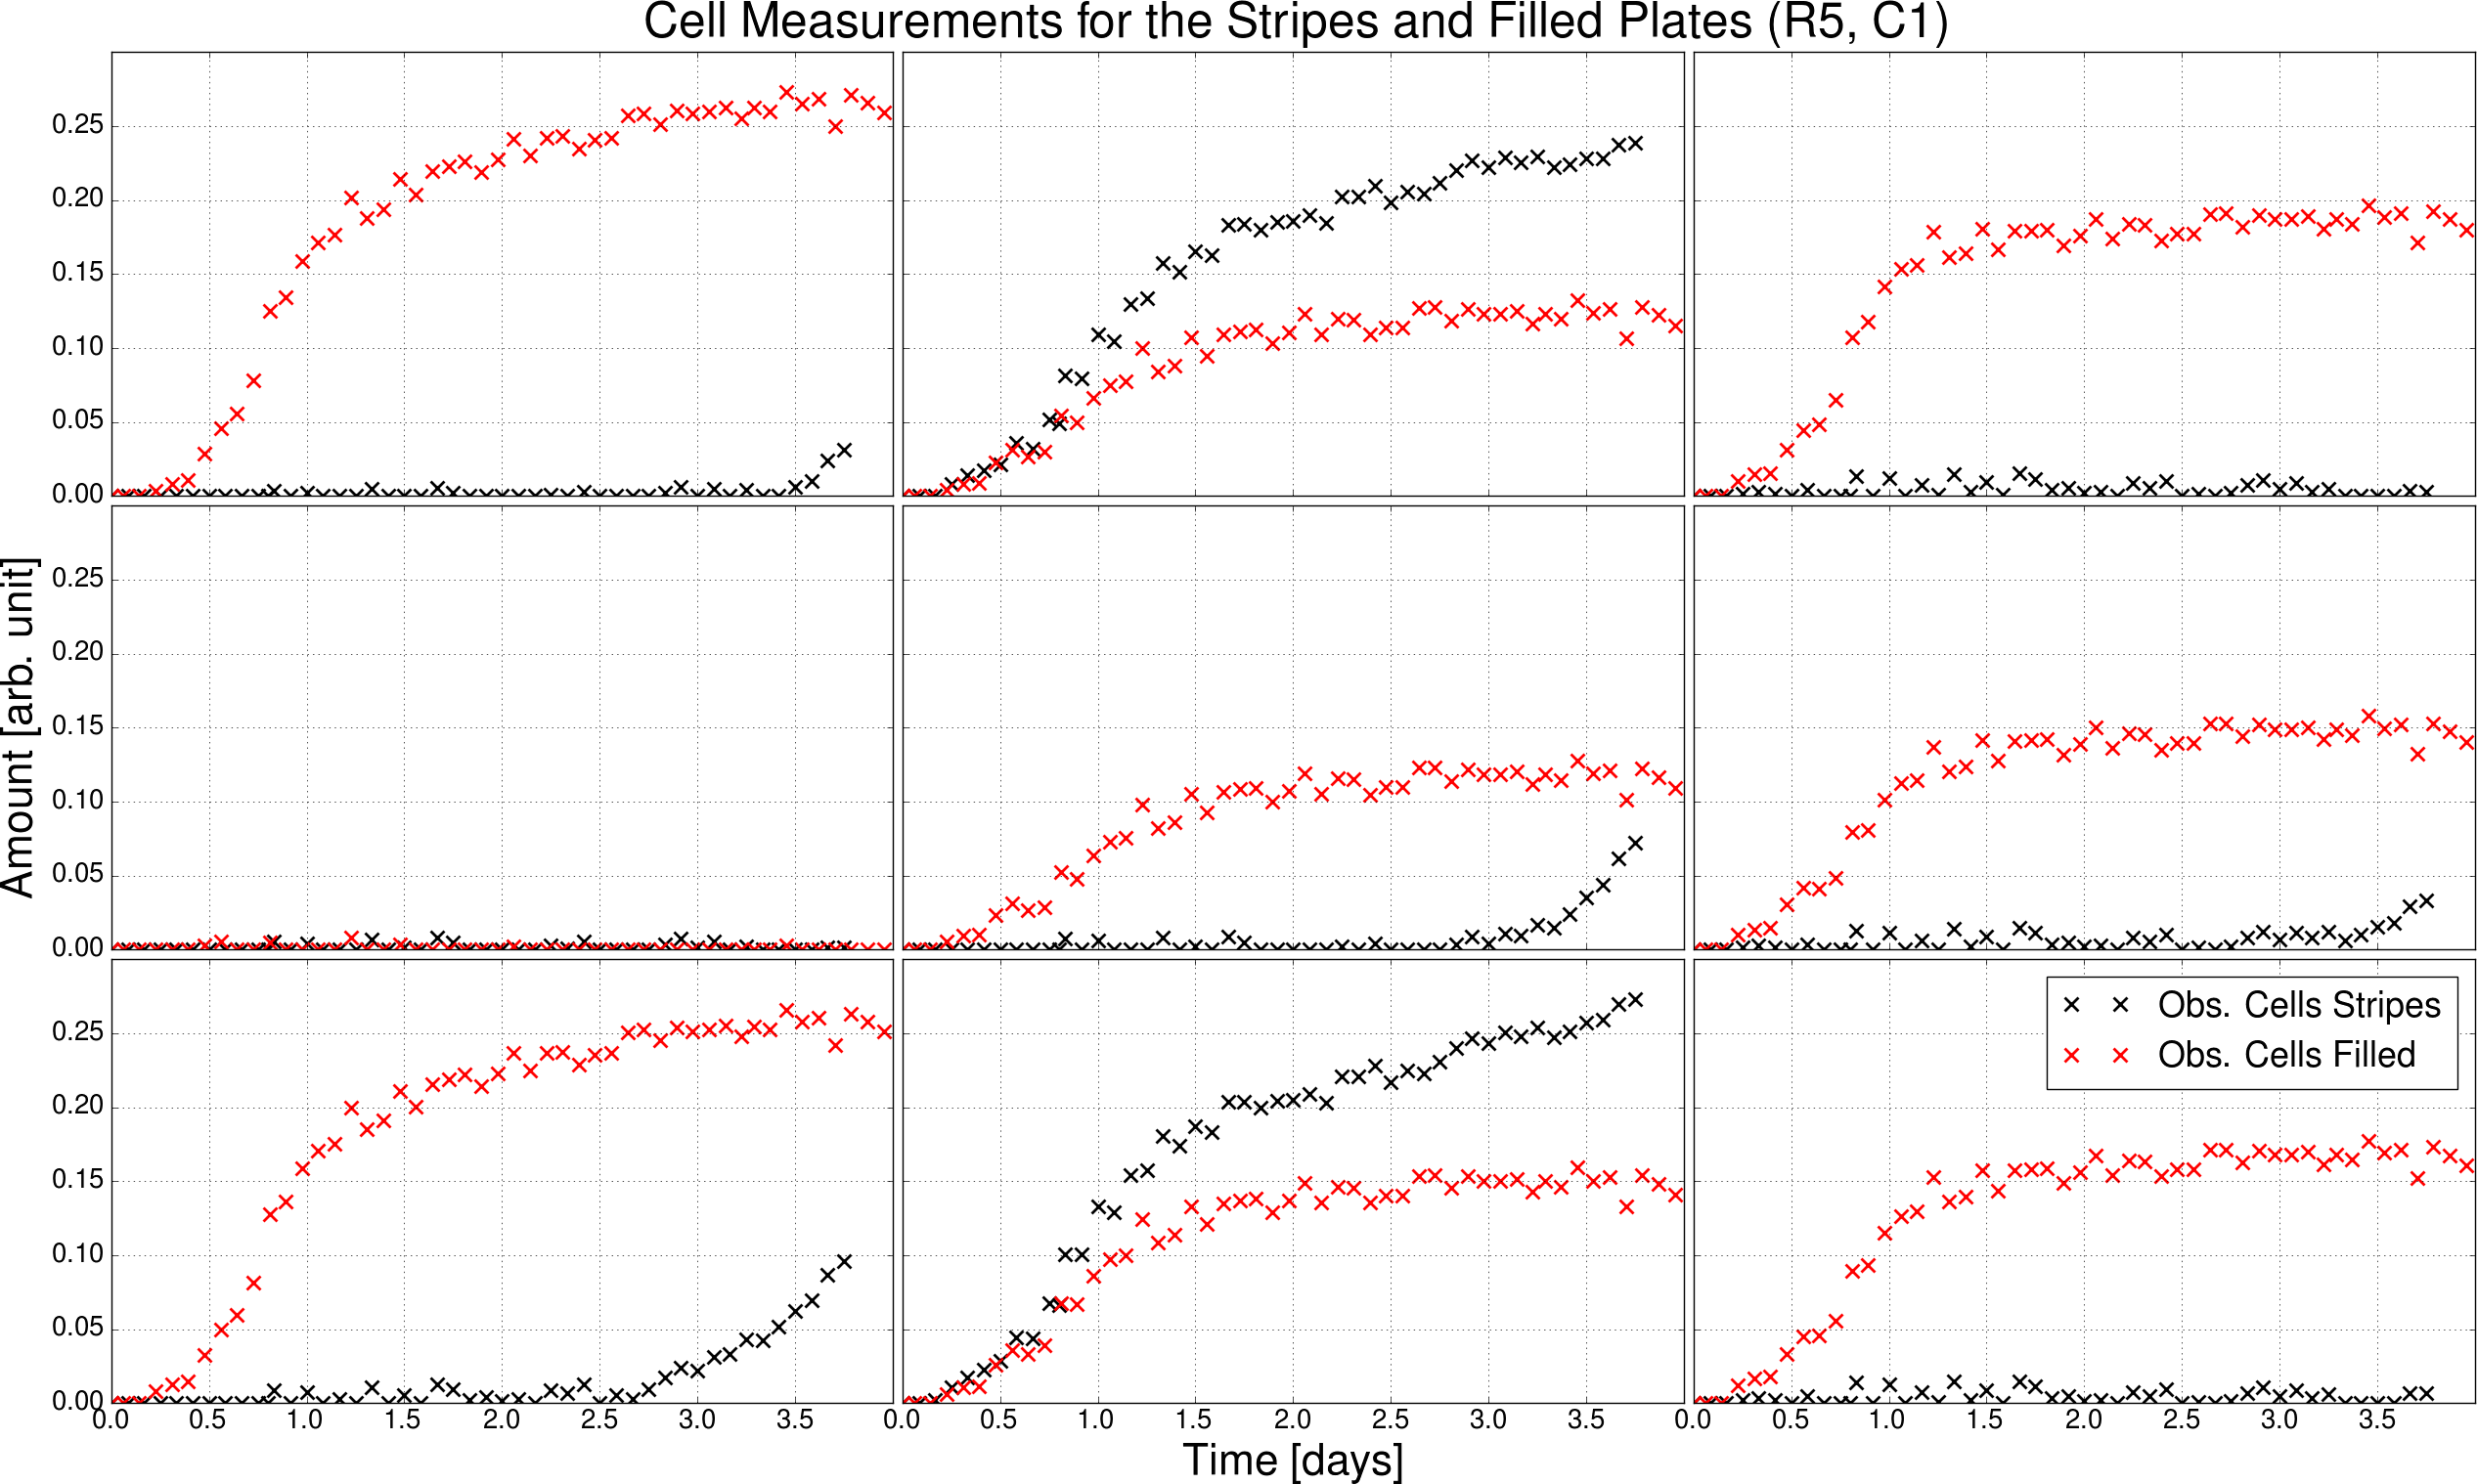
\includegraphics[width=\linewidth]{final/c_meas_r5_c1}
  \captionof{figure}{Observed cells for (R5, C1) 3x3 zone of Stripes
    and Filled plates showing (for Stripes data) slow growing cultures
    starting to grow after faster growing cultures have reached the
    stationary phase.}
  \label{fig:kn_guessing}
\end{Figure}


We have only studied data where cultures are grown in an array on
solid agar where we cannot validate the independent limit. In this
limit, our model says that nutrients can only be converted to cells
and all cultures starting with the same amount of nutrients will reach
the same final cell density. This ignores metabolism which may differ
between strains. Cell arrest could also limit growth. If present,
differences in such effects could account entirely for differences in
final cell density. However, they are unlikely to be the only effect,
because this would not lead to the observed characteristic endpoint in
growth. Using one-culture spot tests (in a perti-dish on ager?) or
liquid cultures we can grow cultures independently and validate the
independent limit. A current issue with methods for estimating
fitness, is that identical strains grow differently on agar or in
liquid culture leading to different fitness rankings (cite). This
problem need not affect our validation as we can simply define a
culture to have different parameters for growth in either medium. A
greater difference may be caused by the dimensionality of the
environment. Mass action kinetics is derived for reactions in a
three-dimentsional (gas or fluid?) (Guldberg and Waage C.M. Guldberg
and P. Waage, Studies Concerning Affinity, C. M. Forhandlinger:
Videnskabs-Selskabet i Christiana (1864), 35) and this approximation
is more valid for liquid cultures than for cultures spotted onto a
surface. I suggest to study first the more ideal case of liquid
cultures and later see if the model holds for cultures grown on a
surface. If it does not, it may be necessary to use a fractal kinetics
model (I have references for this from the proposal) or, if the
reaction is diffusion limited, consider a more detailed model of
nutrient diffusion.

// Model equations for metabolism.//

Reo and Korolev (2014) simulate nutrient dependent growth of a single
bacterial culture on a pertri dish in two-dimensions using the
diffusion equation and Neumann and Dirichlet boundary conditions. They
create a sink for nutrients from culture growth and equate the flux of
nutrients through the culture area with the rate of increase in
culture size. They model culture area as varying and keep culture
density constant. We may instead keep culture area constant, allow
culture density to vary, and use our mass action kinetic model for the
nutrient sink and culture growth. Simulating or fitting this model
could help us learn more about diffusion in QFA experiments. I am
interested to know whether growth becomes diffusion limited at some
time-point (before nutrients are fully depleted) and what area of
nutrients a culture can access within this time. It is probably
unfeasible to use such a detailed model to fit a whole plate because
of the computational time this would take. However, if necessary, it
may be possible to use a finer grid to increase compartmentalisation
of nutrients. This could extend the validity of the competition model
over a larger range of variability in culture growth rates (for
instance when some cultures are left empty and others are very fast
growing.) (Probably a mistake to leave cultures completely empty in
validation plot; should have instead just used weaker growers to
induce a smaller change).

It would also be useful to determine experimentally how nutrients are
distributed throughout the agar at the stationary phase. Gaps could be
left in an array of cultures and only inoculated once the stationary
phase is reached. If they grow then nutrients remain. This could be
extended by growing a single column of identical strains and, after
the stationary stage has been reached, inoculating identical strains
on the same plate at different distances from the row.

//Talk about an improvement to the imaginary neighbour model.//

The composition of nutrients (sugars, nitrogen, etc.) in QFQ agars
follows a traditional recipe designed to reduce the excess of any
single nutrient (check QFA paper and cite). ((background) What is the
nutrient?  Nitrogen is only used to build molecules for new cells,
whereas sugars are also used for metabolism.) For modelling nutrient
limited growth, especially across plates, it would be better if we
knew the identity of the limiting nutrient and could ensure that it is
always the same molecule. This could be achieved using a different
formula of agar.

//Signalling//

If we find that competition for nutrients is not a significant effect,
for instance if growth becomes diffusion limited before nutrients from
neighbours can be accessed, then we could instead model signalling by
ethanol as the interaction effect. This may be modelled similarly to
how we are already modelling nutrient diffusion.

//Signalling equation//

If there is any combination of effects contributing significantly to
differences in the growth of cultures and the interaction between
neighbours then it will be difficult to separate them when fitting a
model to data. We may have to develop ways to calibrate effects in
isolation (e.g. by adding/measuring ethanol?) and use this information
when fitting to high-throughput data.

It is quicker to fit to small zones of a plate but as these have a
larger proportion of edge cultures boundary conditions become
important. In current data (e.g. P15) the cultures surrounding the
edge may be very different from each other and this makes accurate
fitting difficult. As a result we need to use larger zones are more
difficult to work with. If we could surround small 3x3 and 4x4 zones
with an empty ring then we would only need to consider the net flux of
nutrients into or out of the zone and not the variation cultures
surrounding the zone. We could also surround with an identical strain
to reduce net flux although then we would have to consider biological
variance.
% (Would it be better not to use a temperature dependent strain?)
//

Stochastic effects. Unpublished work by Hermann and Lawless has
investigated heterogeneity between cell lines within single QFA
spots. They have found that a single or small number of extremely fast
growing cell-lines can come to dominate the population of a single
culture. The implication is that cultures with a lower starting cell
densities are likely to have greater variance between repeats. We
could use higher starting cell concentrations to reduce this variance
but then we study less of the growth phase. It may be possible to
reduce the effect by taking cells to be inoculated from the
exponential growth phase rather than the stationary phase and still
study full growth curves. (Unless mean population growth constant is
being studied...) Staring cell densities should ideally be as close to
the lowest resolvable level as possible.

//Ways to measure C_0//
There is a confounding effect between initial cell density and

To fit growth curves more accurately QFA has begun using the
generalised logistic model. General logistic model shows higher
coeffient of variation in estimated (MDR*MDP or MDR) than either the
standard logistic model or competition model.


//Improvement to imaginary neighbour guessing//

% also talk about computational limitations of more complicated
% modelling approaches. Can do this when describing the motivation for
% the fought for model.

\subsection{\thesubsection~Subsection}

%%% Local Variables:
%%% mode: latex
%%% TeX-master: "report"
%%% End:
